\documentclass{article}
\usepackage[utf8]{inputenc}
%% Sets page size and margins
\usepackage[a4paper,top=2cm,bottom=2cm,left=2cm,right=2cm,marginparwidth=1.75cm]{geometry}

\usepackage{algorithm}
\usepackage{algorithmic}
\usepackage{float}
\renewcommand{\algorithmicrequire}{ \textbf{Input:}} %Use Input in the format of Algorithm
\renewcommand{\algorithmicensure}{ \textbf{Output:}} %UseOutput in the format of Algorithm
\usepackage{multirow}
%\usepackage{fdsymbol}
\usepackage{amsthm}
%% Useful packages
\usepackage{amsmath}
\usepackage{amssymb}
\usepackage{latexsym}
%\usepackage{fdsymbol} 
\usepackage{ dsfont }
\usepackage{color}
\usepackage{bm}
\usepackage{graphicx}
\usepackage[export]{adjustbox}
\usepackage[colorinlistoftodos]{todonotes}
\usepackage[colorlinks=true, allcolors=blue]{hyperref}
\usepackage{biblatex}
\addbibresource{references.bib}

\title{Plots of Subgradient}
%\author{Wei Kuang}
%\date{June 29, 2023}

\begin{document}

\maketitle
\section{ADMM}
The objective function is
\begin{equation}
    f(\beta) = \frac{1}{2}\|z-M_{\perp}\beta\|^2 + \lambda\|\beta\|_1,
\end{equation}
thus the subgradient we care about is
\begin{equation}
    \partial f(\beta) = M_{\perp}^T(M_{\perp}\beta-z) + \lambda \partial \|\beta\|_1.
\end{equation}

\begin{figure}[H]
	\centering
	\subfigure{
		\begin{minipage}[b]{1\textwidth}
			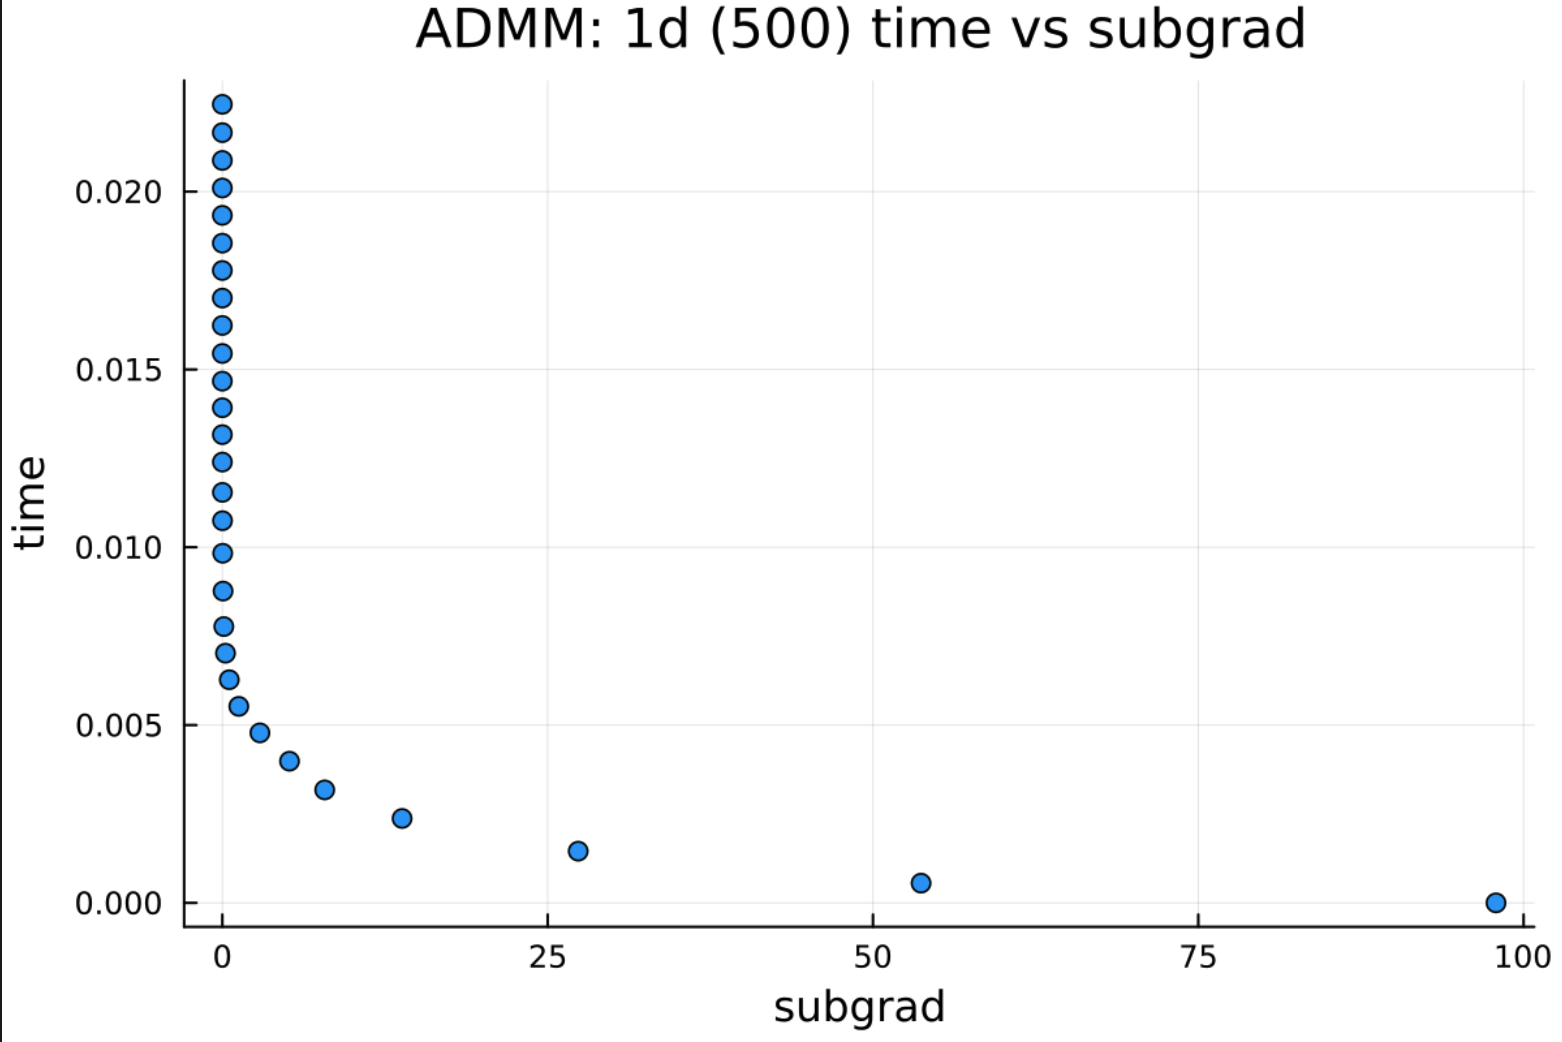
\includegraphics[width=0.3\textwidth]{Interior Point Method/subgradplot3_fig/ADMM1dtimevsgrad.png} 			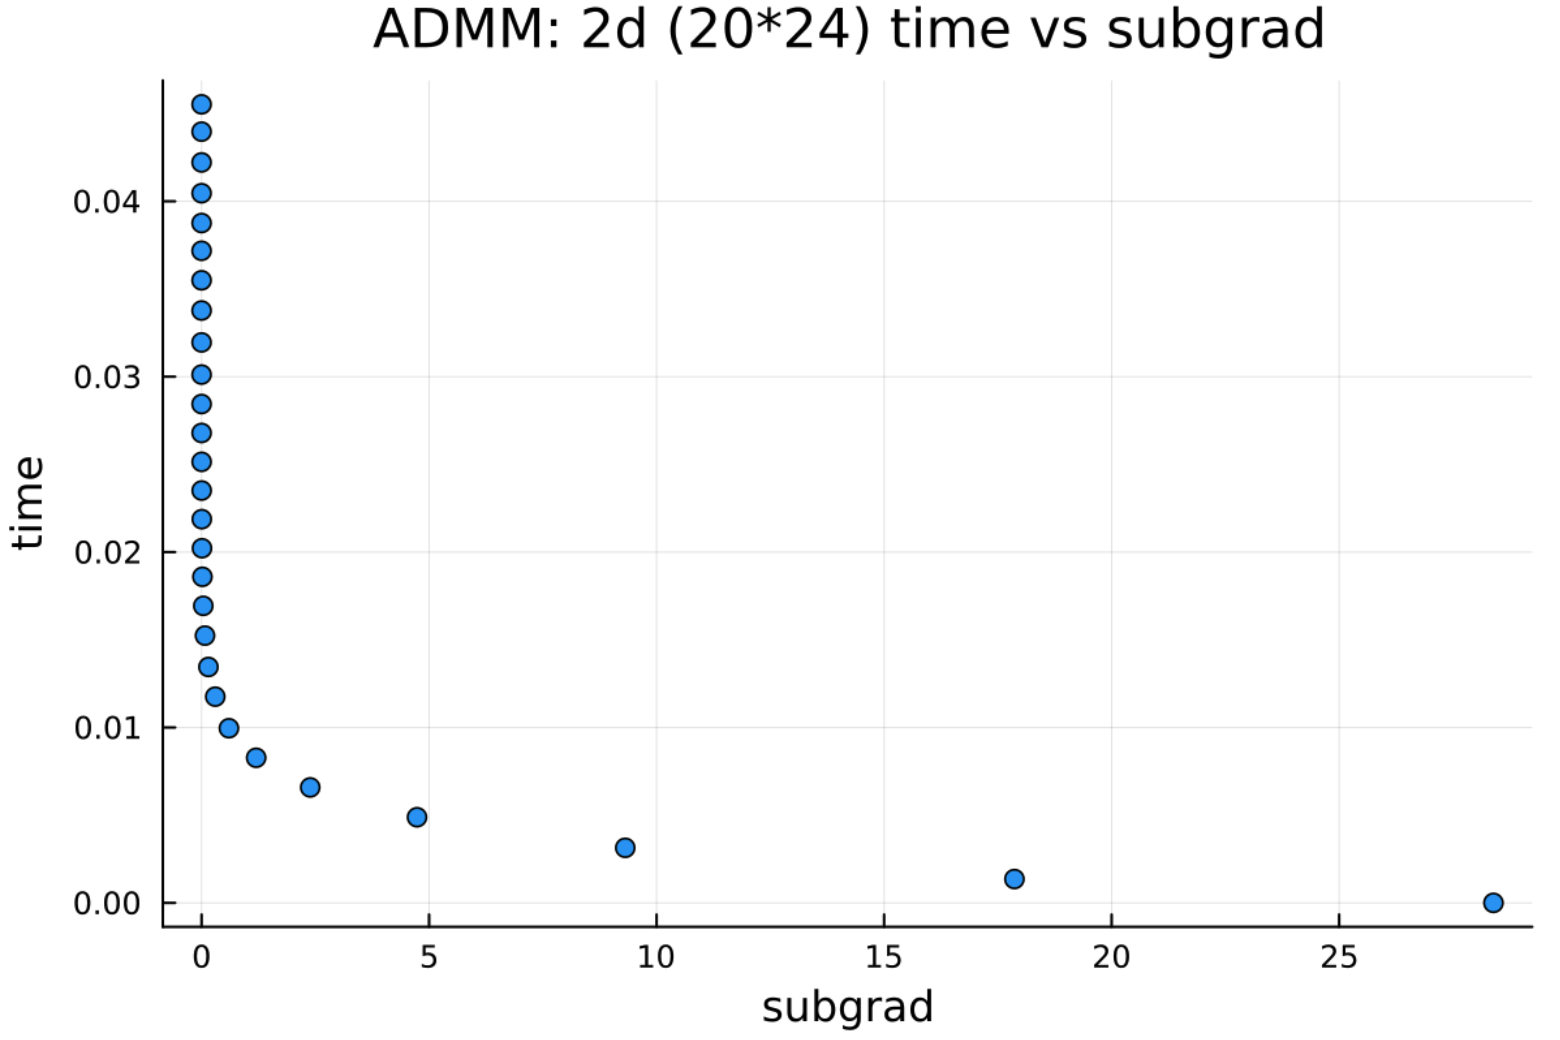
\includegraphics[width=0.3\textwidth]{Interior Point Method/subgradplot3_fig/ADMM2dtimevsgrad.png}
          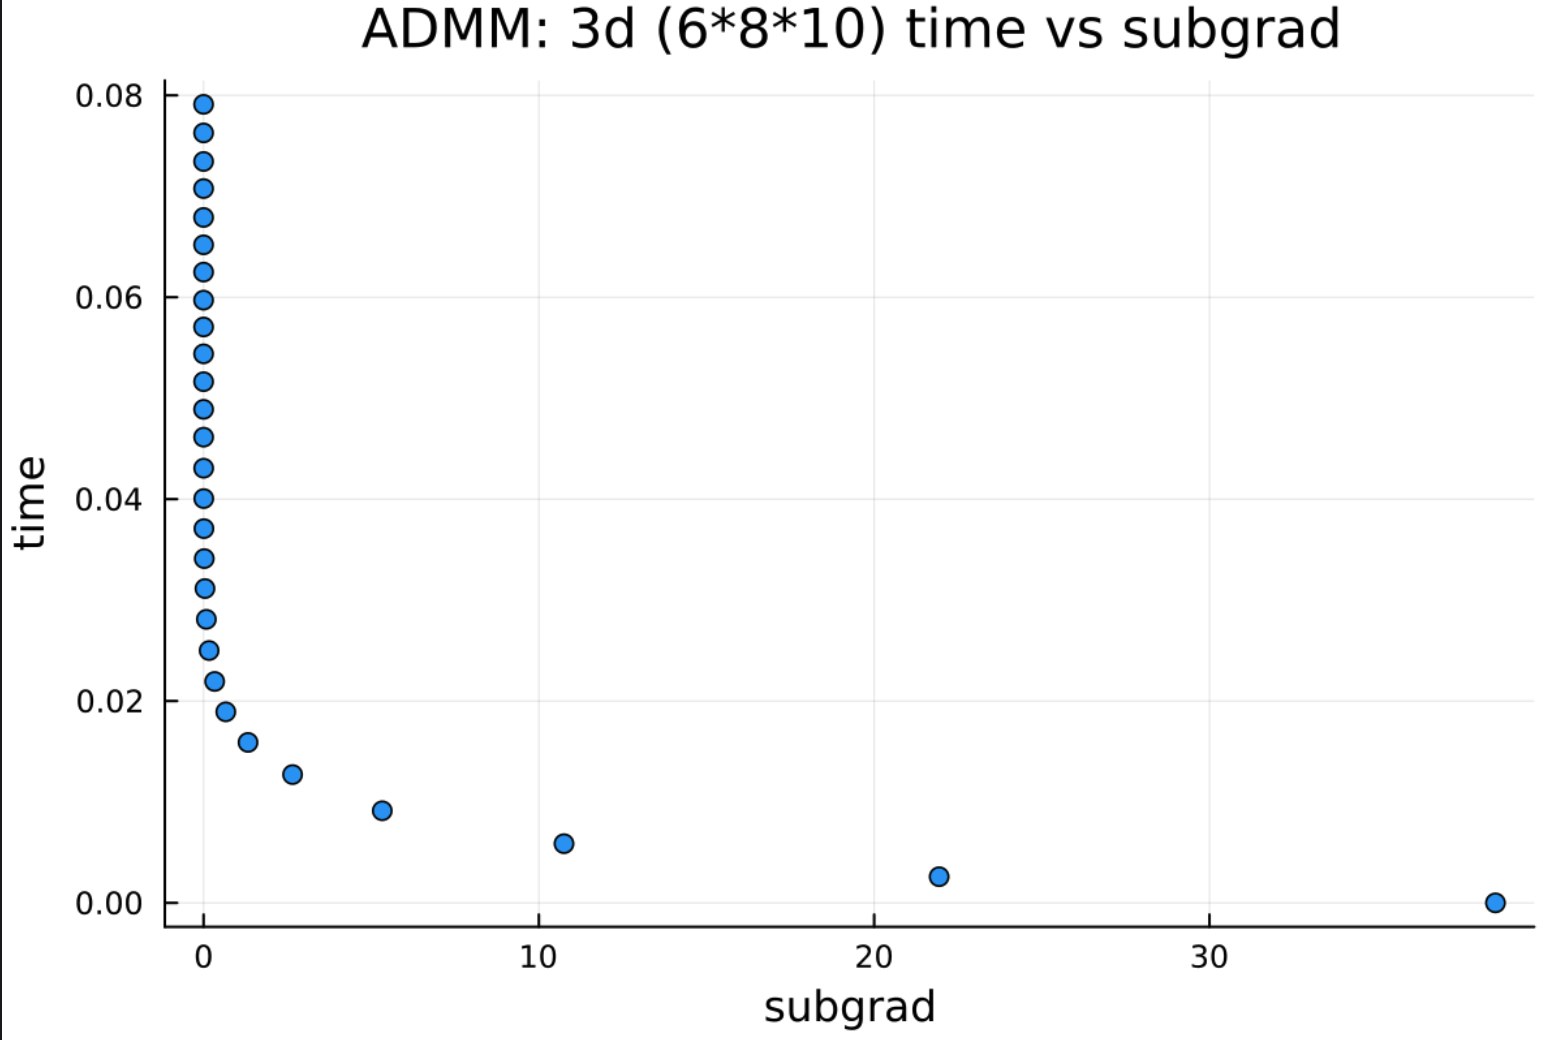
\includegraphics[width=0.3\textwidth]{Interior Point Method/subgradplot3_fig/ADMM3dtimevsgrad.png}
		\end{minipage}
  \caption{ADMM: cumulated time vs subgrad}
	}
    	\subfigure{
    		\begin{minipage}[b]{1\textwidth}
   		 	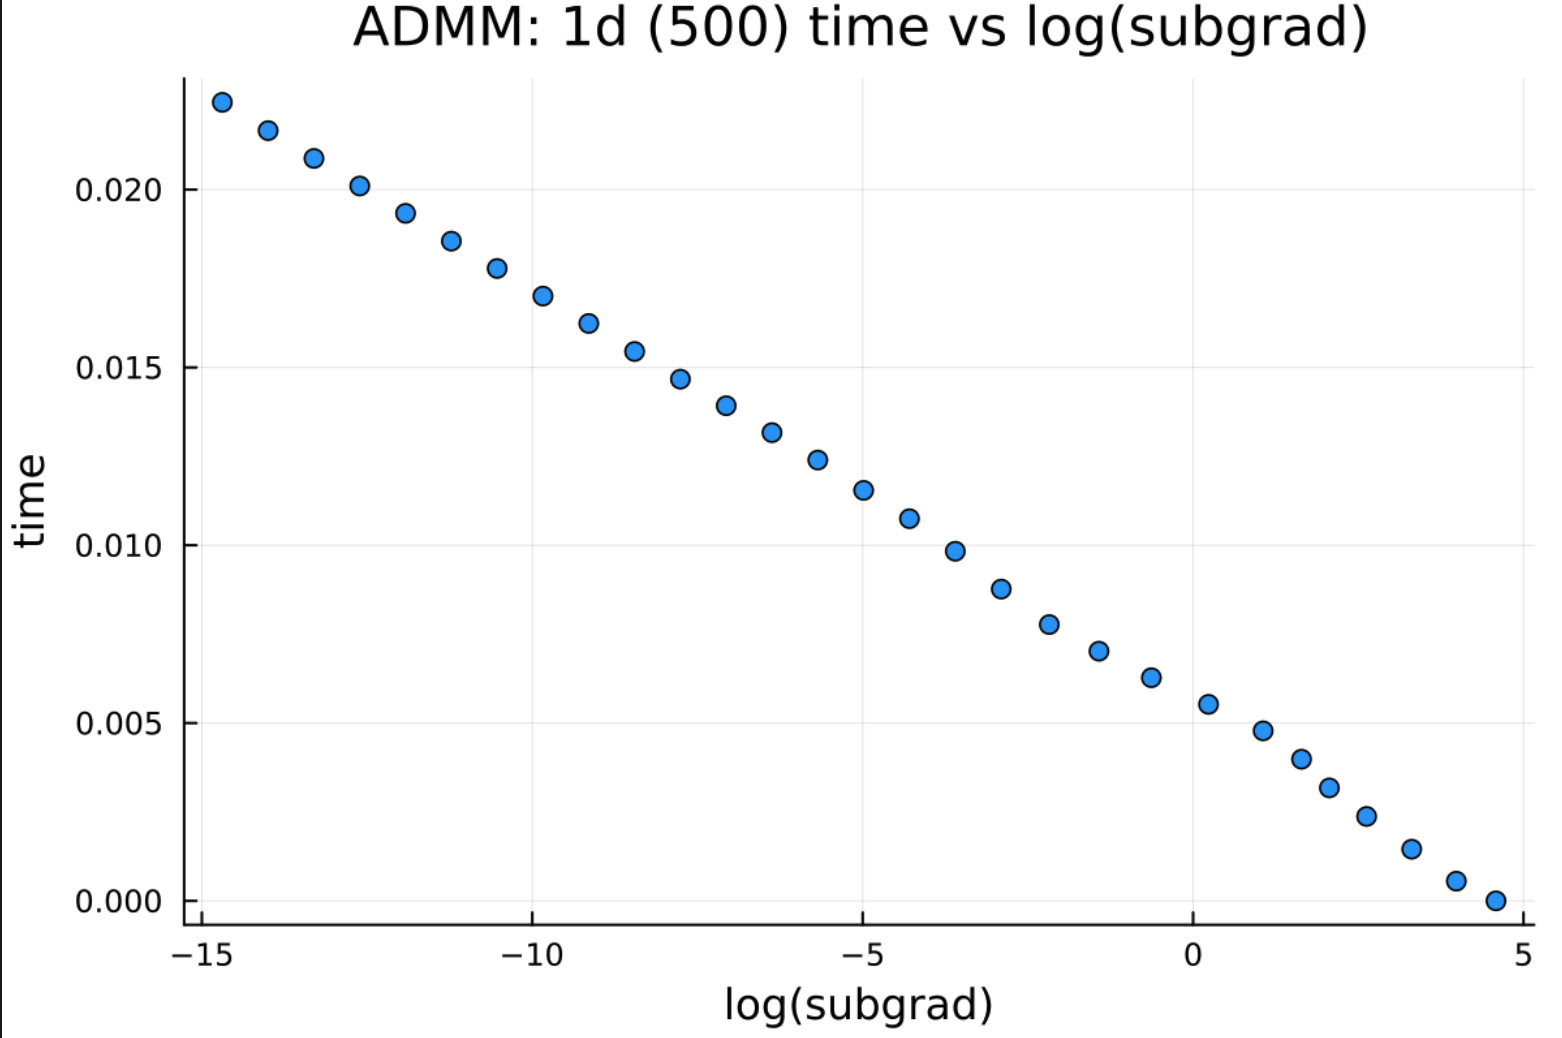
\includegraphics[width=0.3\textwidth]{Interior Point Method/subgradplot3_fig/ADMM1dtimevsloggrad.png}		 	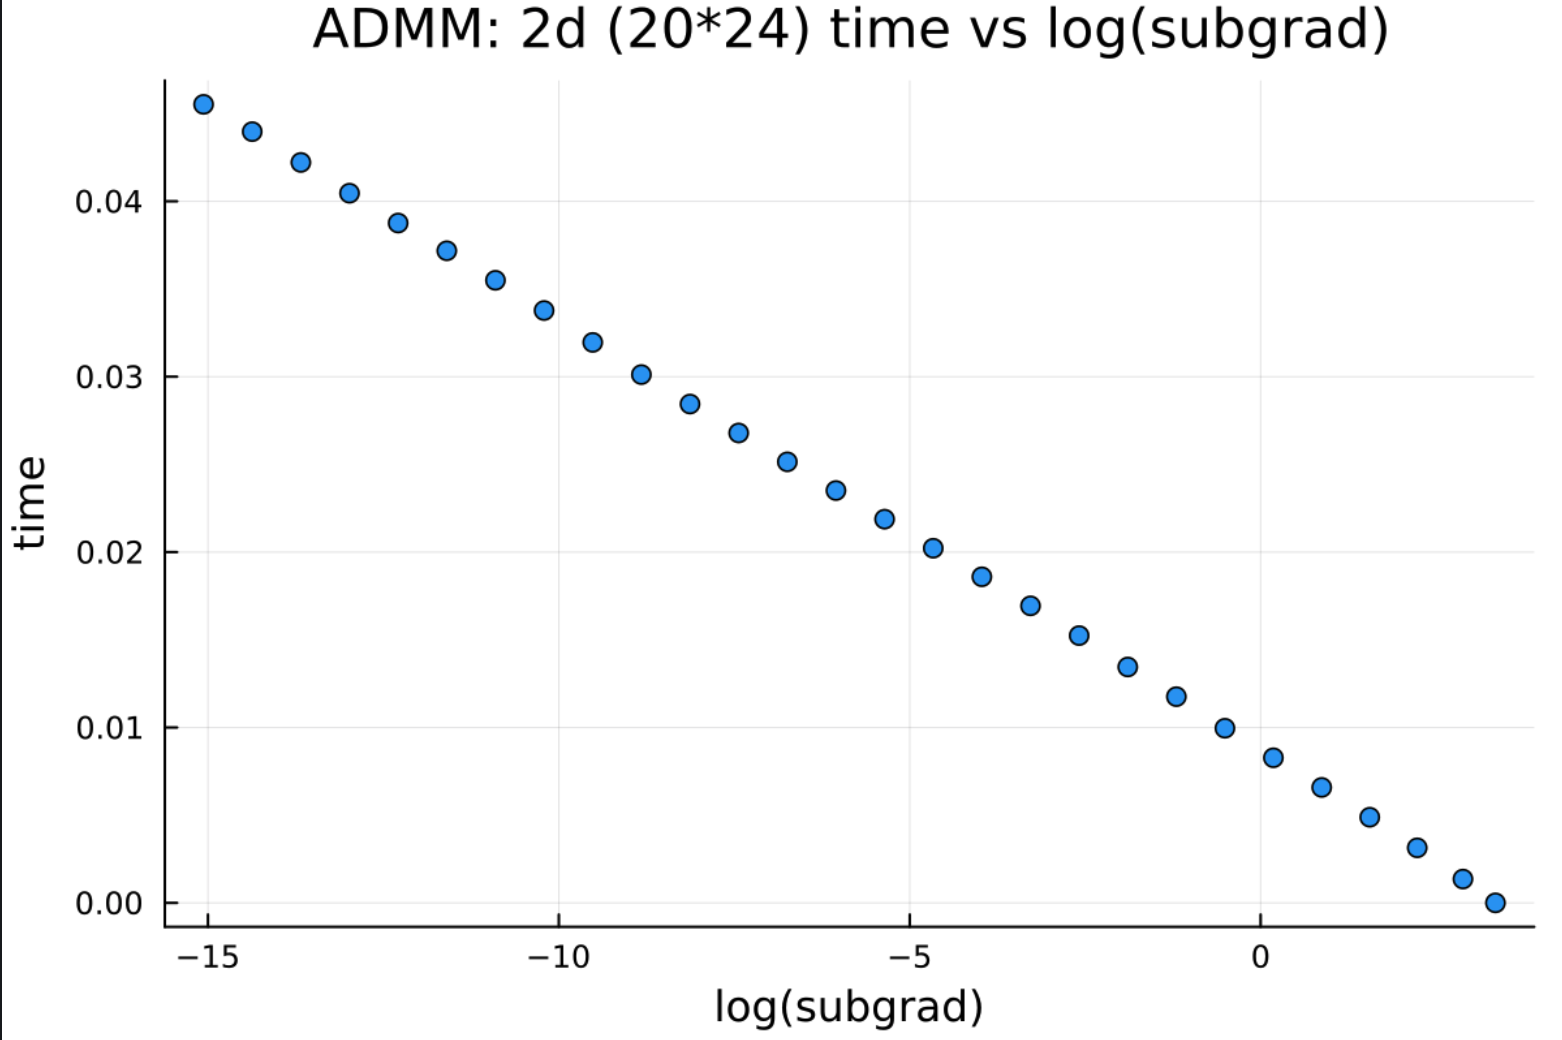
\includegraphics[width=0.3\textwidth]{Interior Point Method/subgradplot3_fig/ADMM2dtimevsloggrad.png}           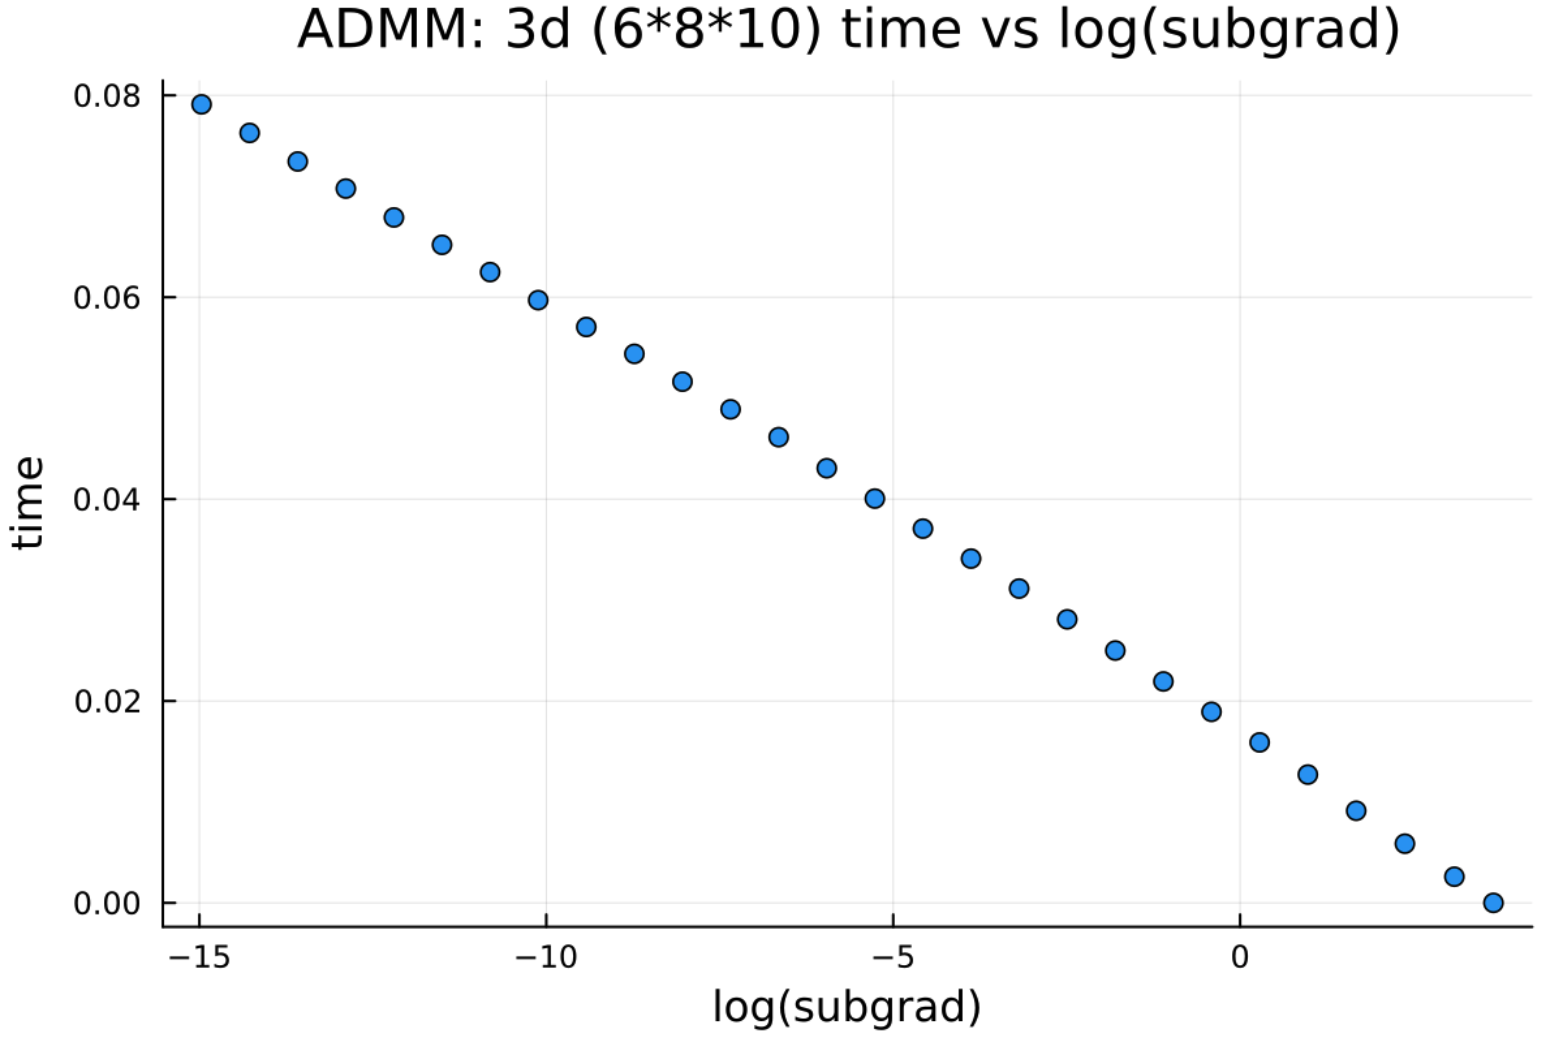
\includegraphics[width=0.3\textwidth]{Interior Point Method/subgradplot3_fig/ADMM3dtimevsloggrad.png}
    		\end{minipage}
      \caption{ADMM: cumulated time vs log(subgrad)}
		}
   	\subfigure{
    		\begin{minipage}[b]{1\textwidth}
   		 	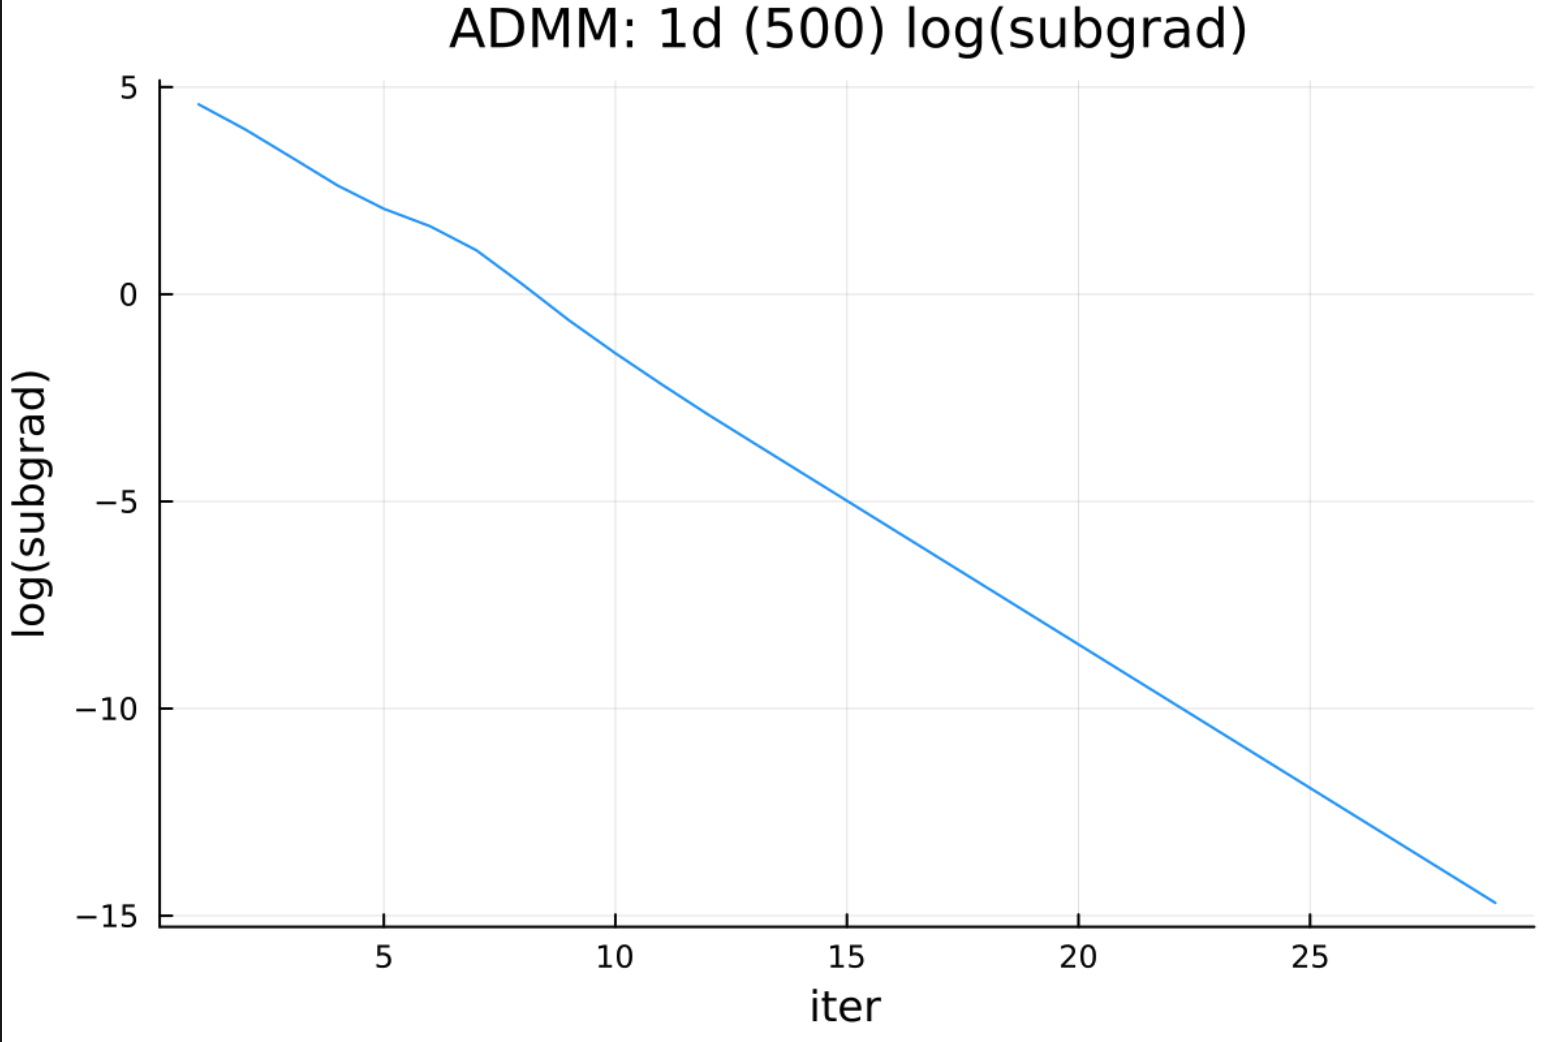
\includegraphics[width=0.3\textwidth]{Interior Point Method/subgradplot3_fig/ADMM1dloggrad.png}		 	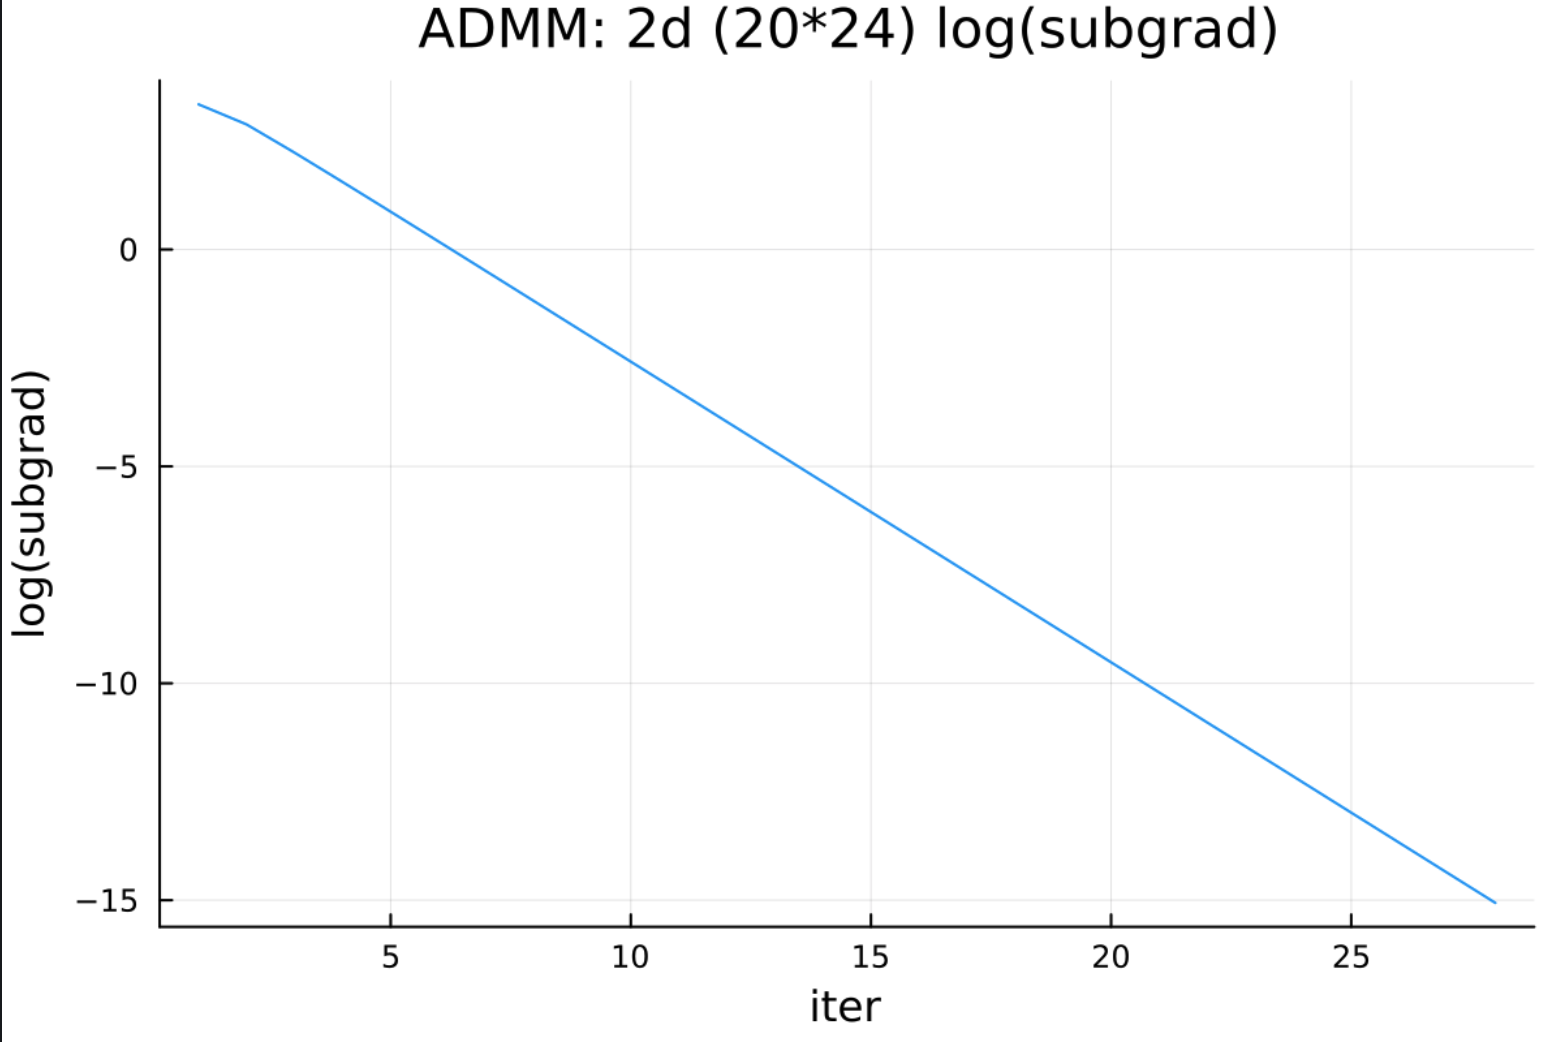
\includegraphics[width=0.3\textwidth]{Interior Point Method/subgradplot3_fig/ADMM2dloggrad.png}           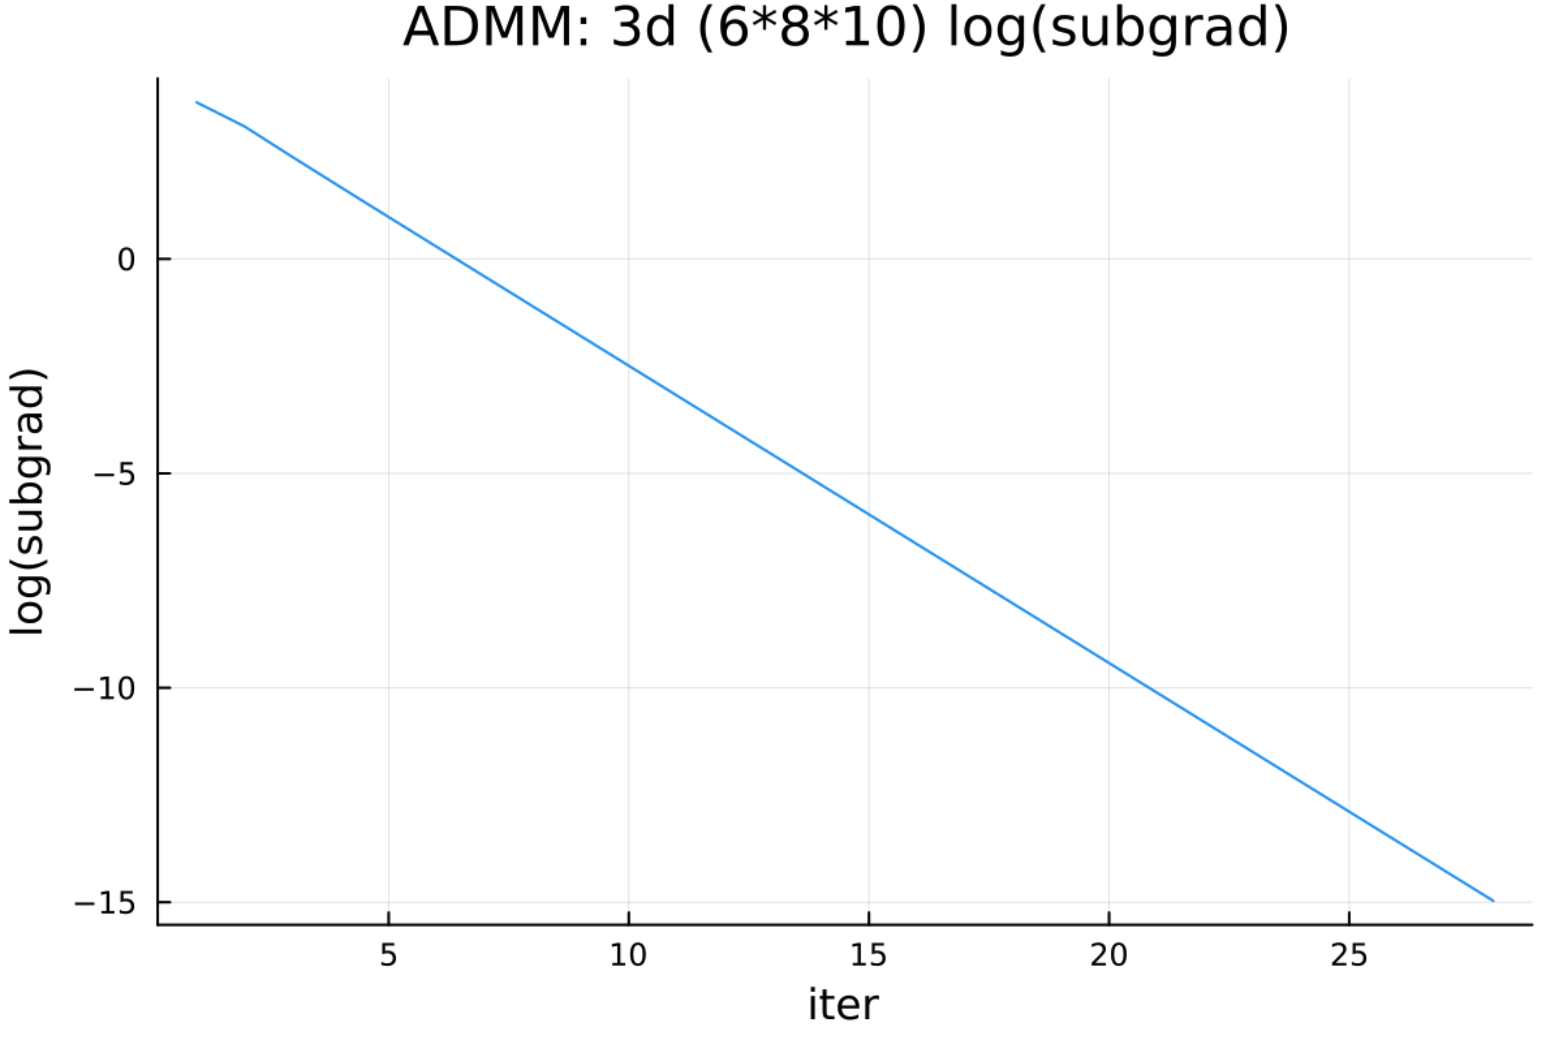
\includegraphics[width=0.3\textwidth]{Interior Point Method/subgradplot3_fig/ADMM3dloggrad.png}
    		\end{minipage}
      \caption{ADMM: log(subgrad) vs iter}
		}  
\end{figure}

\section{IPOPT}
We start with the problem
\begin{equation}
    \min_{\beta} \frac{1}{2}\|z-M_{\perp}\beta\|^2 +\lambda\|\beta\|_1.
\end{equation}
To make the constraint differentiable, we rewrite the problem as
\begin{equation}
    \begin{aligned}
        \min_{\beta, c} &f_0(\beta, c)\frac{1}{2}\|z-M_{\perp}\beta\|^2+\lambda\sum_{i=1}^n c_i\\
        \text{s.t. }&l_i(\beta, c) = -\beta_i-c_i\leq 0\\
        &u_i(\beta, c) = \beta_i-c_i\leq 0
        \end{aligned}
\end{equation}
The log barrier function is
\begin{equation}
    \phi(\beta, c) = -\sum_{i=1}^n\log(-l_i(\beta,c))-\sum_{i=1}^n\log(-u_i(\beta,c)).
\end{equation}
The objective funtcion is
\begin{equation}
    \psi(\beta, c) = t f_0(\beta, c)+\psi(\beta, c).
\end{equation}
We compute the gradient and Hessian of $\psi$.
\begin{equation}
    \nabla\psi(\beta, c) = \begin{pmatrix}
        tM_{\perp}^TM_{\perp}\beta-tM_{\perp}^Tz+\frac{1}{l}-\frac{1}{u}\\
        t\lambda\boldsymbol{1}+\frac{1}{l}+\frac{1}{u}
    \end{pmatrix},\quad
    \nabla^2\psi(\beta,c)=\begin{pmatrix}
        tM_{\perp}^TM_{\perp}+diag\big(\frac{1}{l^2}+\frac{1}{u^2}\big) &diag\big(\frac{1}{l^2}-\frac{1}{u^2}\big)\\
        diag\big(\frac{1}{l^2}-\frac{1}{u^2}\big)
        &diag\big(\frac{1}{l^2}+\frac{1}{u^2}\big).
    \end{pmatrix}
\end{equation}
We need to solve the linear system
\begin{equation}
    \nabla^2 \psi(\beta,c)\begin{pmatrix}
        \Delta \beta\\
        \Delta c
    \end{pmatrix} = -\nabla \psi(\beta, c).
\end{equation}
We use preconditioned CG to solve the linear system. The algorithm is as follows.
\begin{figure}[H]
\centering
   		 	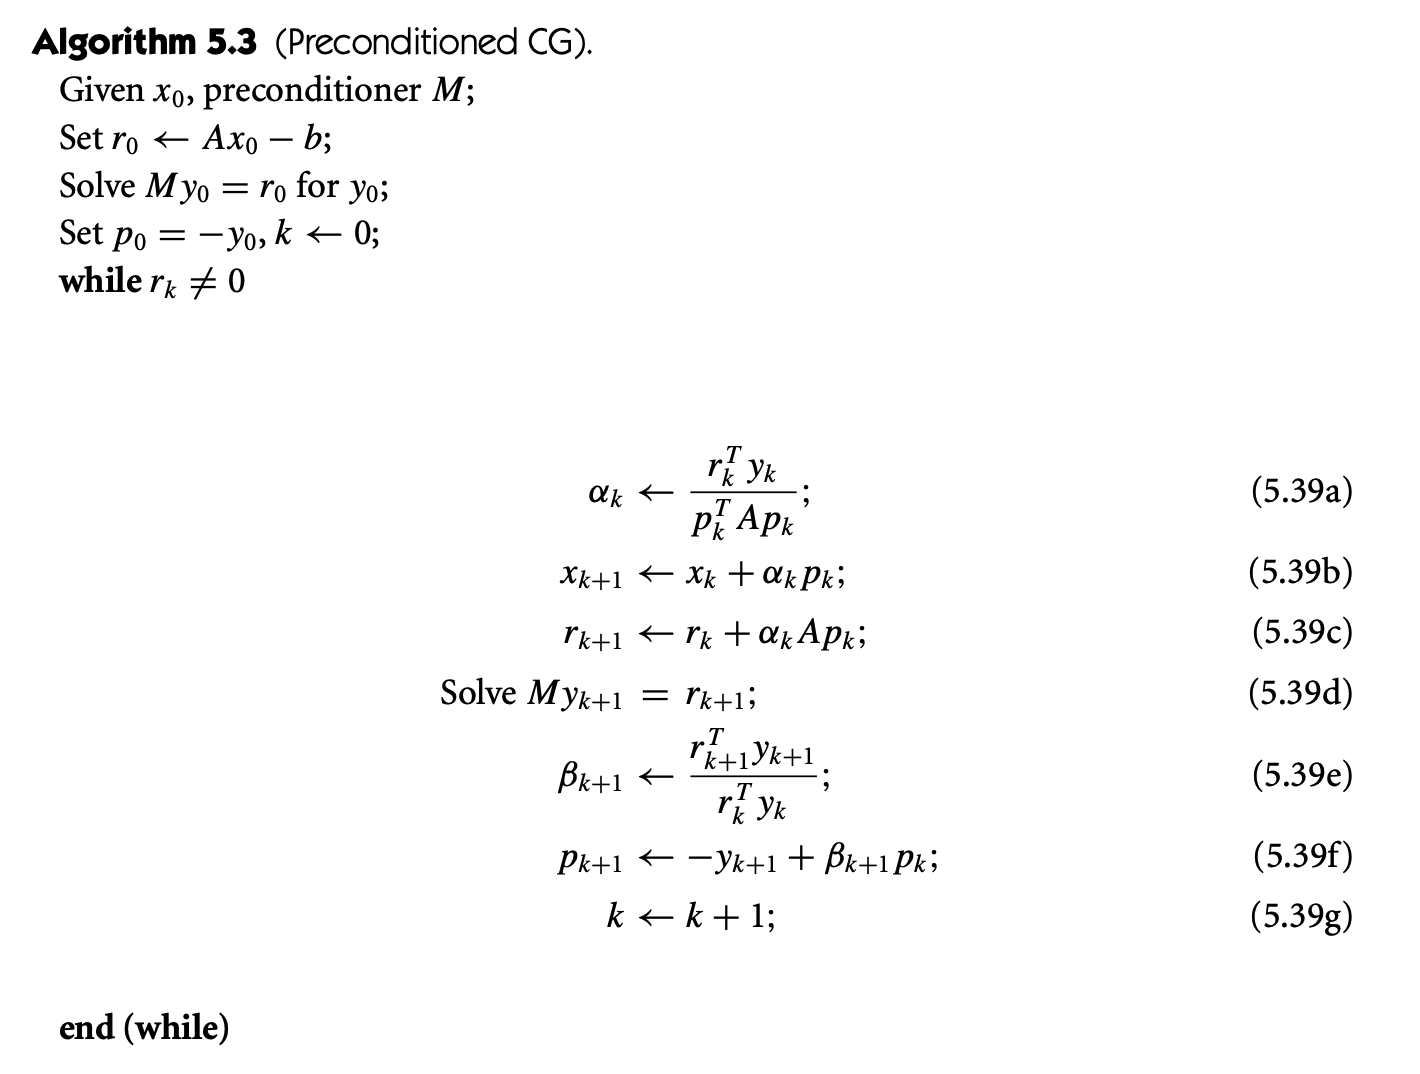
\includegraphics[width=0.8\textwidth]{Interior Point Method/subgradplot3_fig/preconditionedCG.png}		 	
      \caption{preconditioned CG algorithm}
\end{figure}
The preconditioner is chosen as ($M$ is notation abused. Here it is the preconditioner, not the missing rows.)
\begin{equation}
    M = \begin{pmatrix}
        tI 
+ diag\big( \frac{1}{l^2}+\frac{1}{u^2}\big) &diag\big(\frac{1}{l^2}-\frac{1}{u^2}\big)\\
        diag\big(\frac{1}{l^2}-\frac{1}{u^2}\big)
        &diag\big(\frac{1}{l^2}+\frac{1}{u^2}\big).
    \end{pmatrix}
\end{equation}
The subgradient we record is the same as ADMM:
\begin{equation}
    M_{\perp}^T(M_{\perp}\beta-z) + \lambda \partial \|\beta\|_1.
\end{equation}
The following are the plots.
\begin{figure}[H]
	\centering
	\subfigure{
		\begin{minipage}[b]{1\textwidth}
			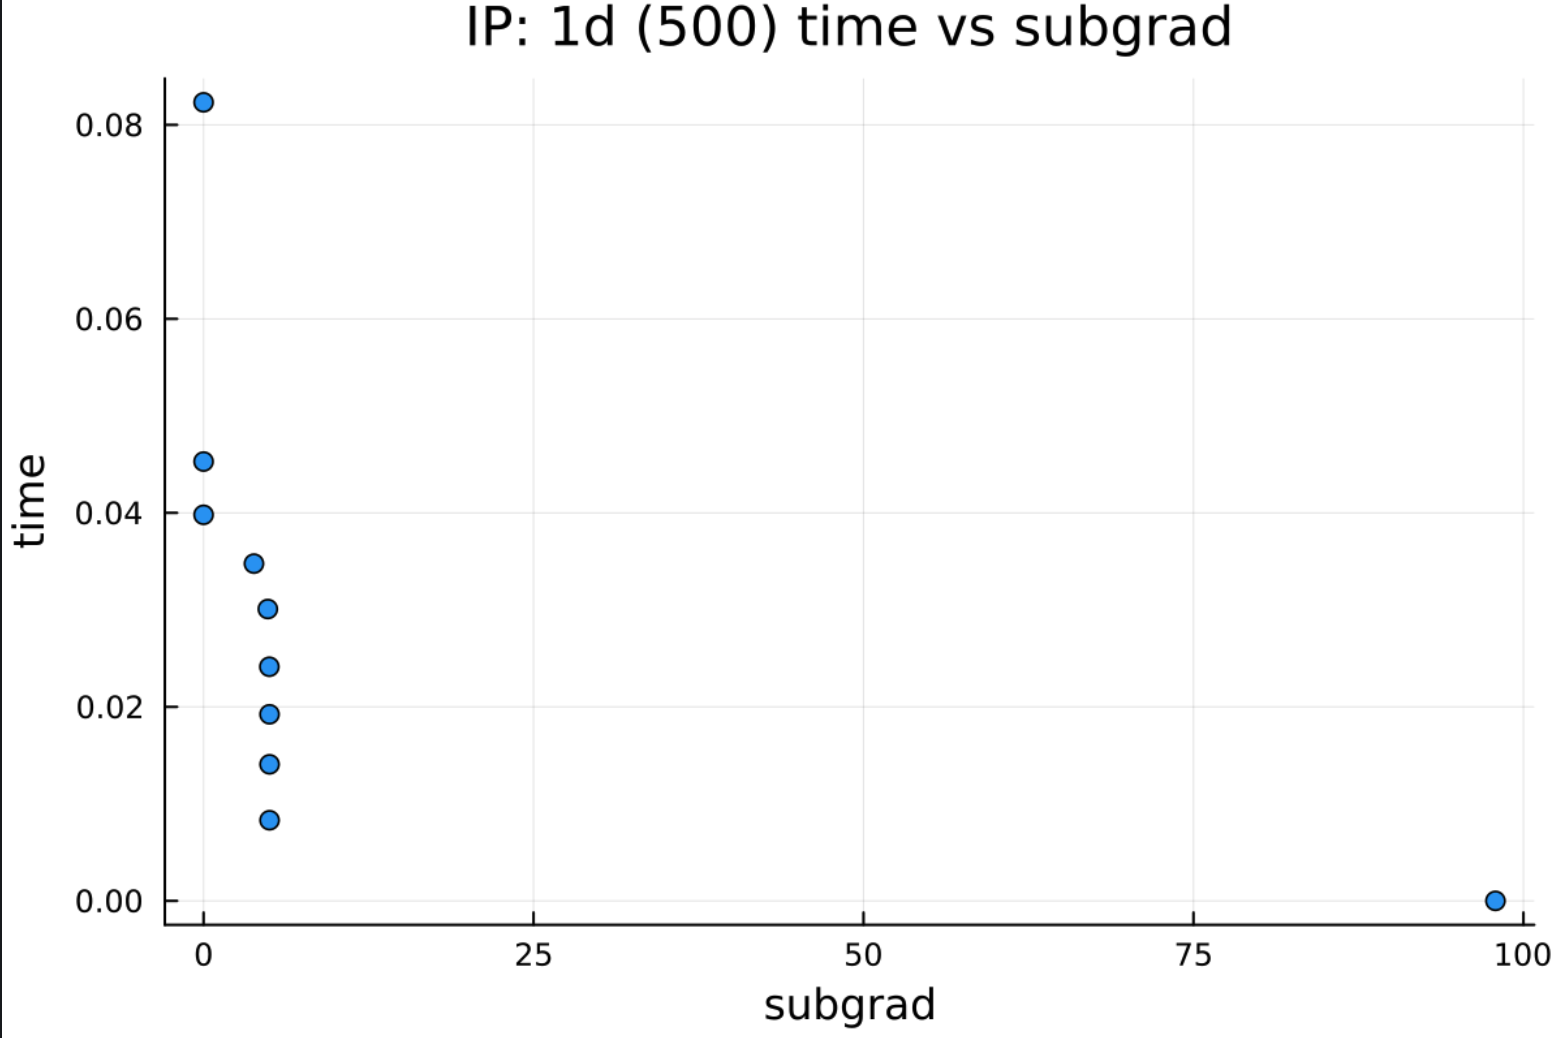
\includegraphics[width=0.3\textwidth]{Interior Point Method/subgradplot3_fig/IP1dtimevsgrad.png} 			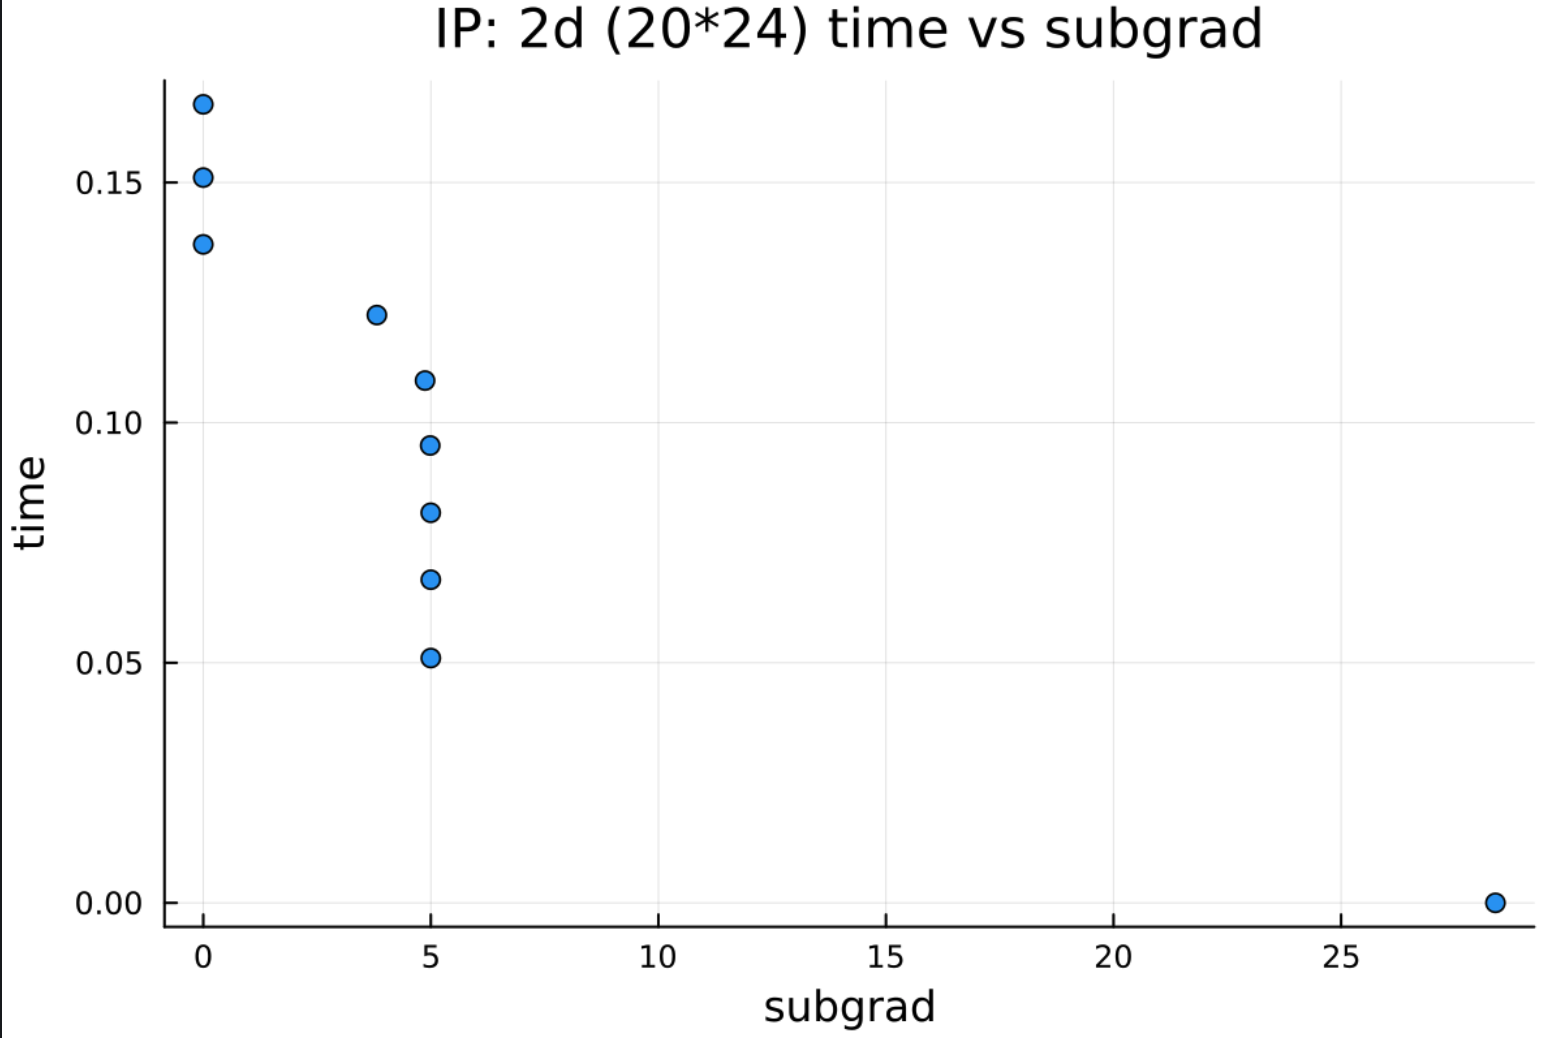
\includegraphics[width=0.3\textwidth]{Interior Point Method/subgradplot3_fig/IP2dtimevsgrad.png}
          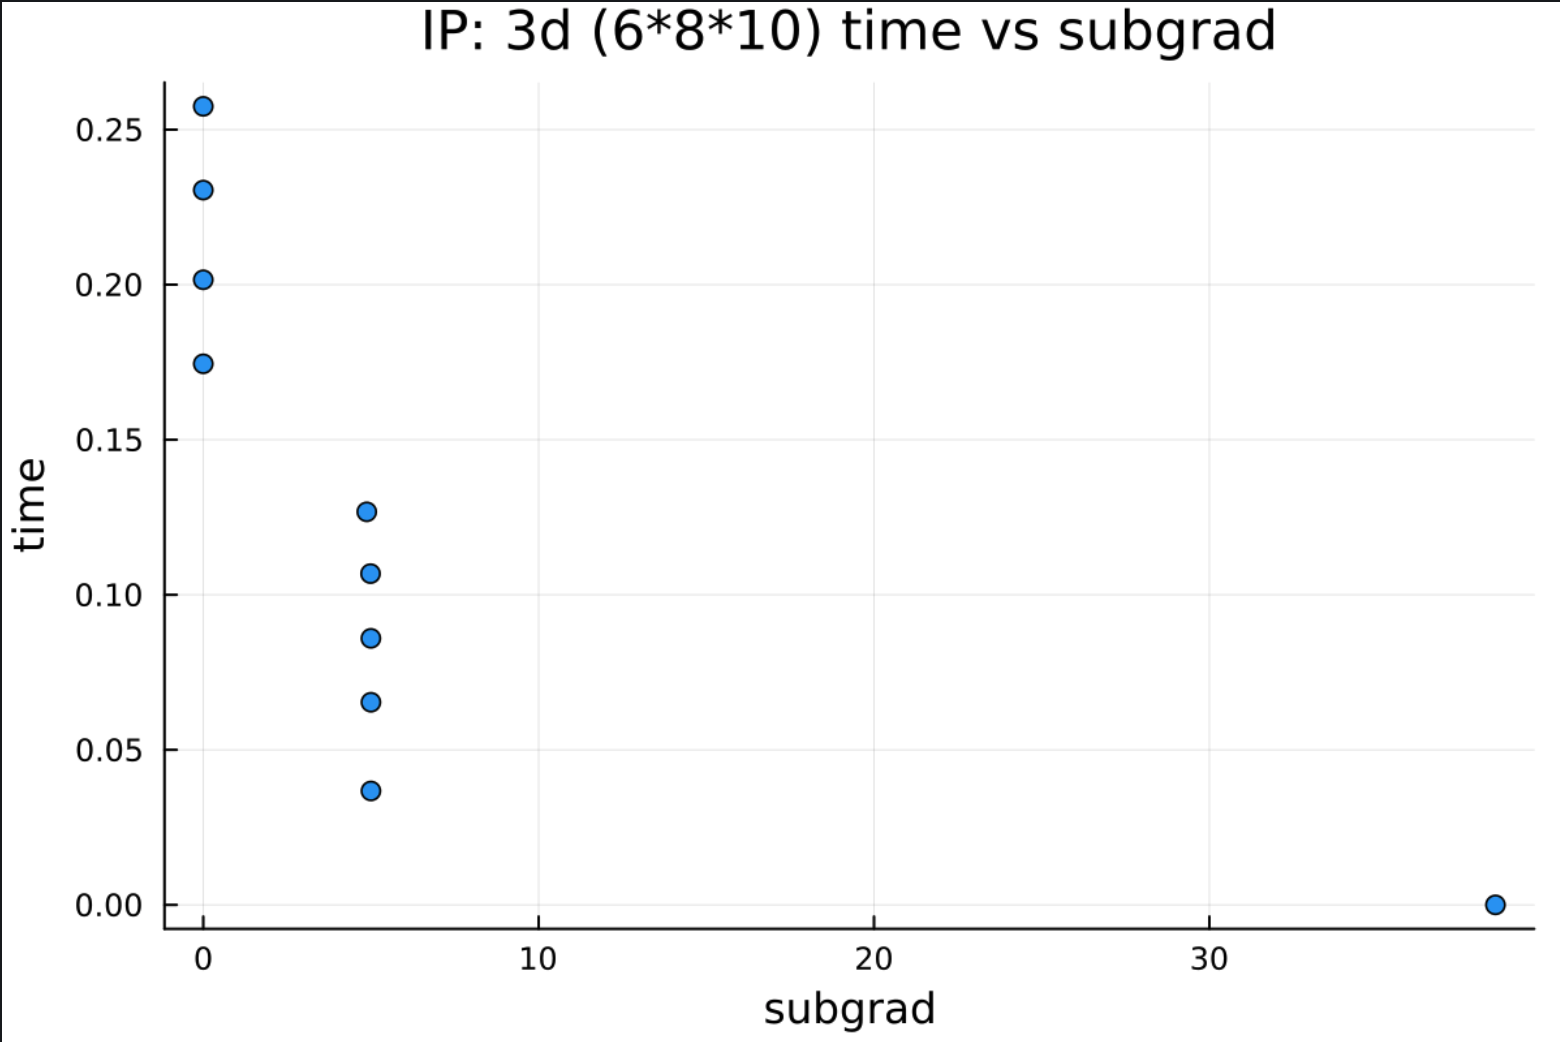
\includegraphics[width=0.3\textwidth]{Interior Point Method/subgradplot3_fig/IP3dtimevsgrad.png}
		\end{minipage}
  \caption{IP: cumulated time vs subgrad}
	}
    	\subfigure{
    		\begin{minipage}[b]{1\textwidth}
   		 	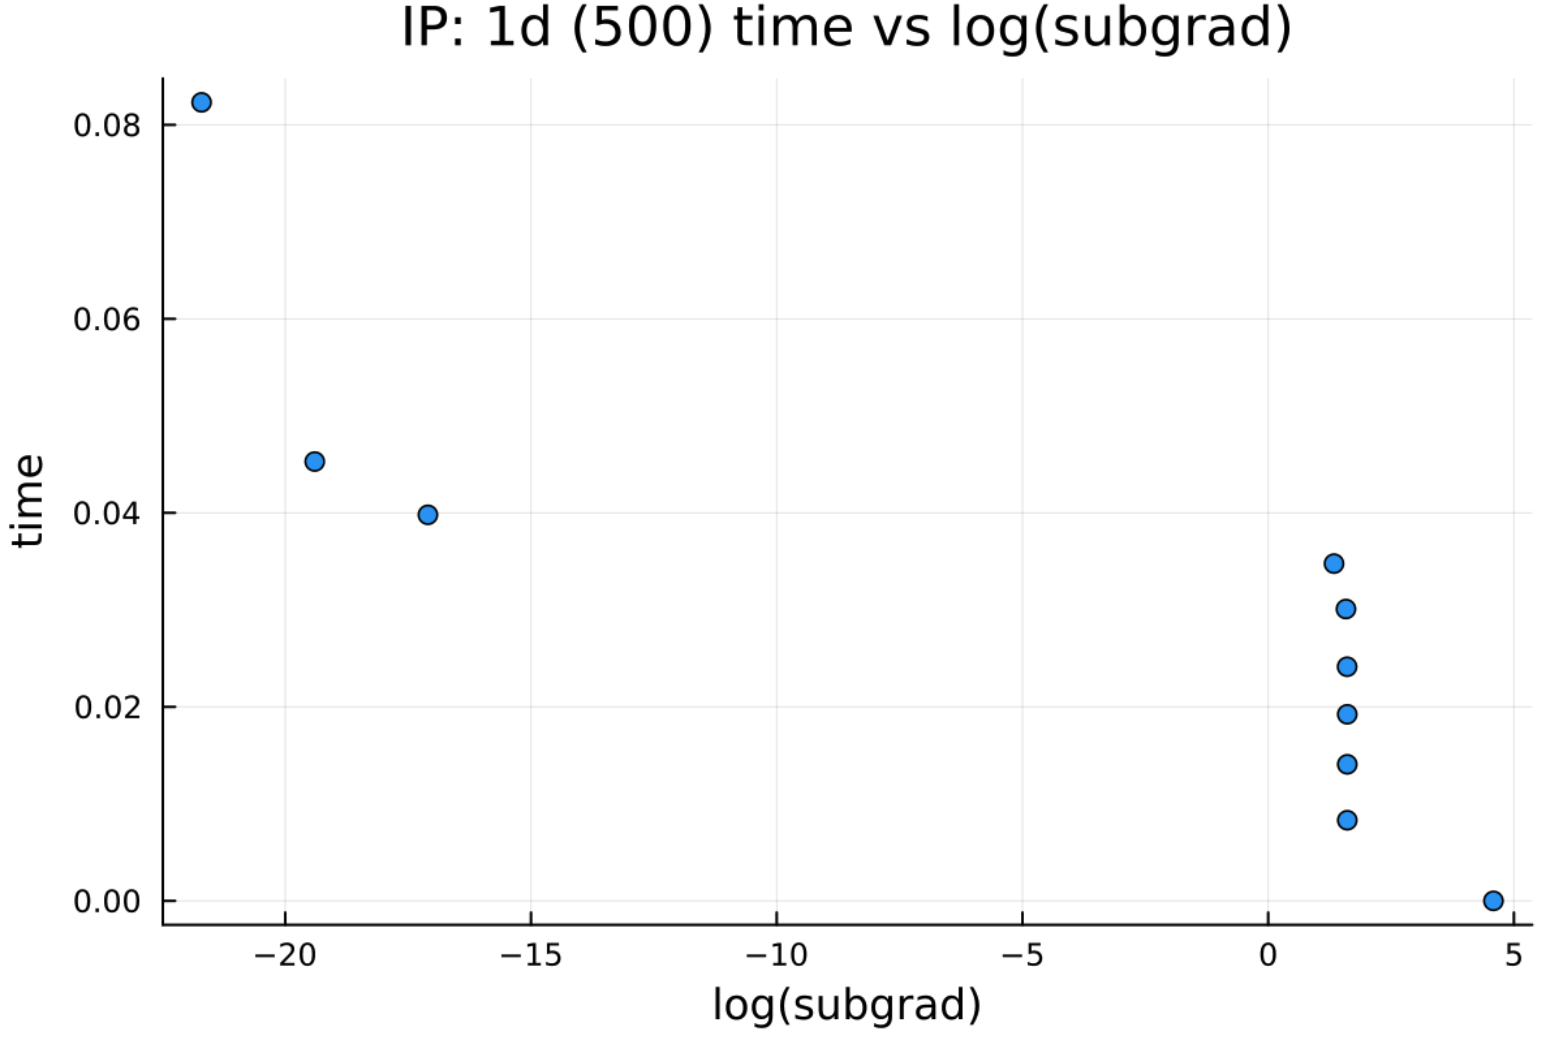
\includegraphics[width=0.3\textwidth]{Interior Point Method/subgradplot3_fig/IP1dtimevsloggrad.png}		 	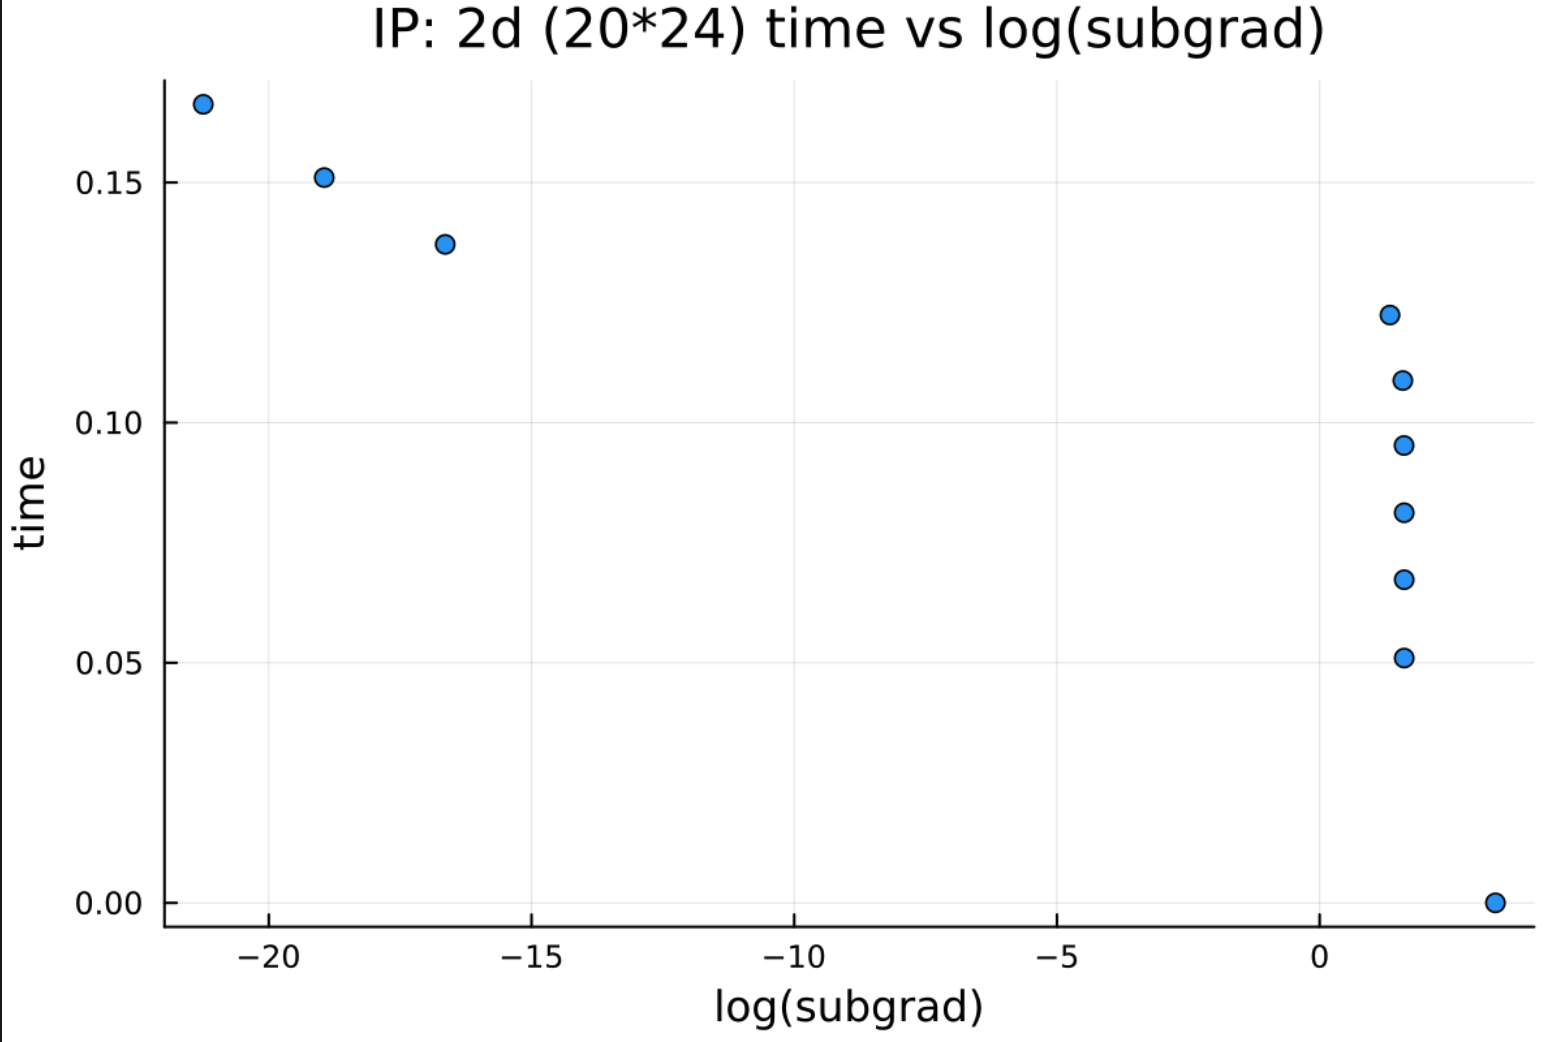
\includegraphics[width=0.3\textwidth]{Interior Point Method/subgradplot3_fig/IP2dtimevsloggrad.png}           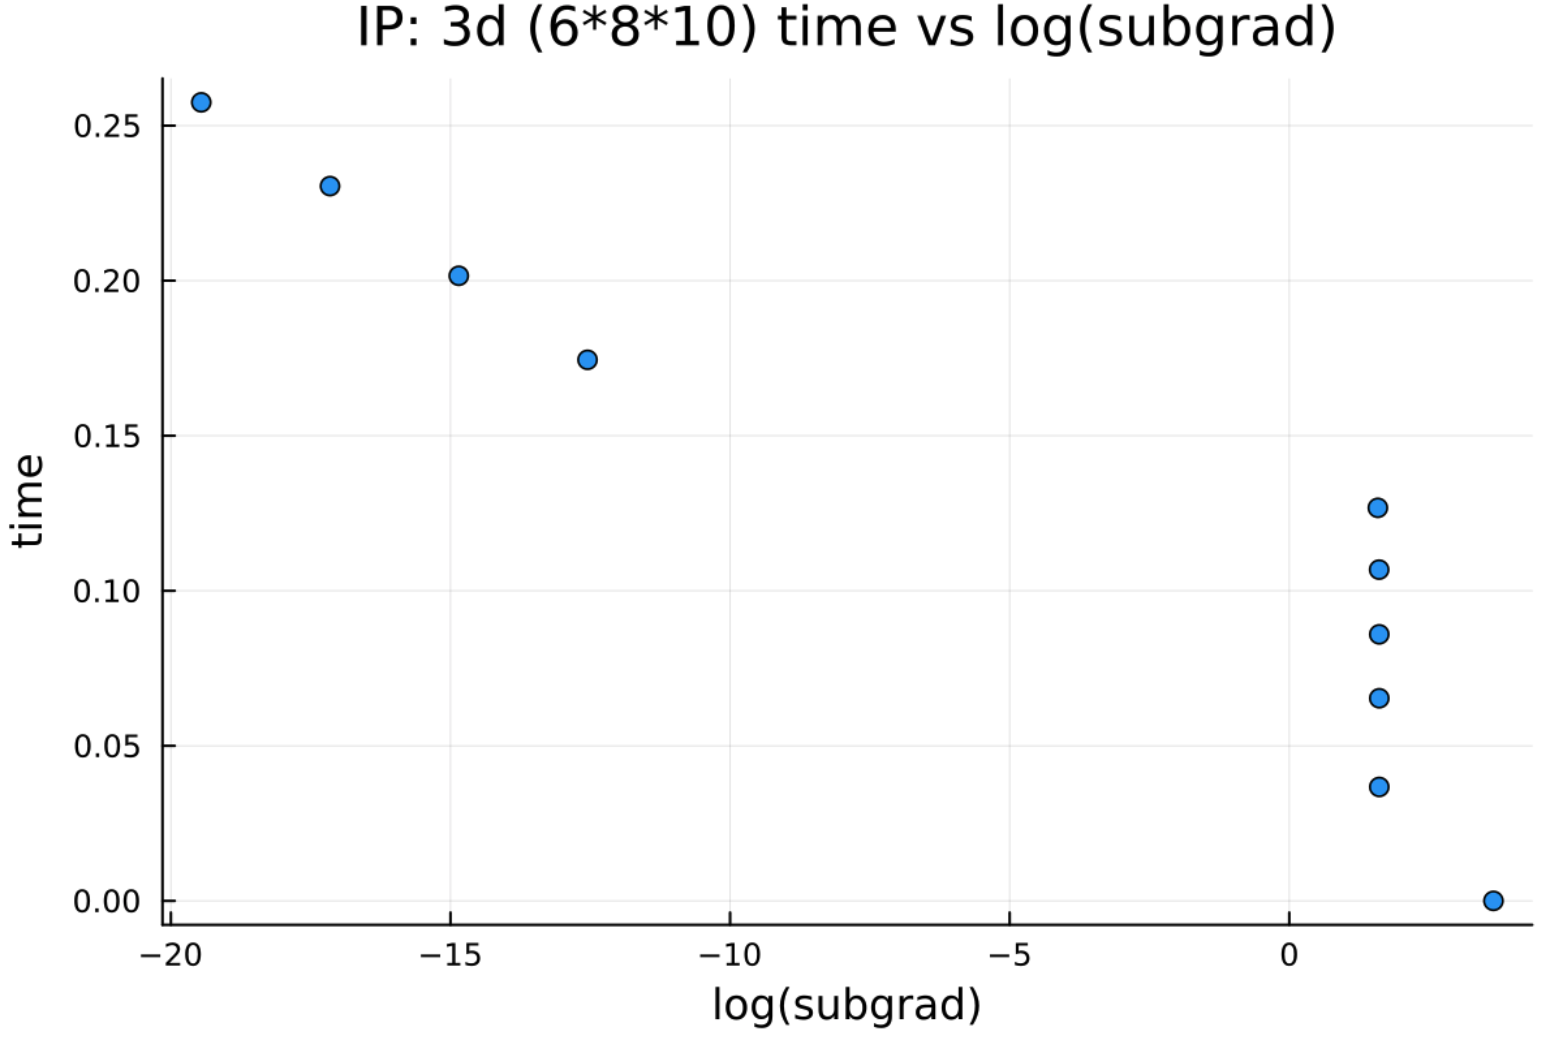
\includegraphics[width=0.3\textwidth]{Interior Point Method/subgradplot3_fig/IP3dtimevsloggrad.png}
    		\end{minipage}
      \caption{IP: cumulated time vs log(subgrad)}
		}
   	\subfigure{
    		\begin{minipage}[b]{1\textwidth}
   		 	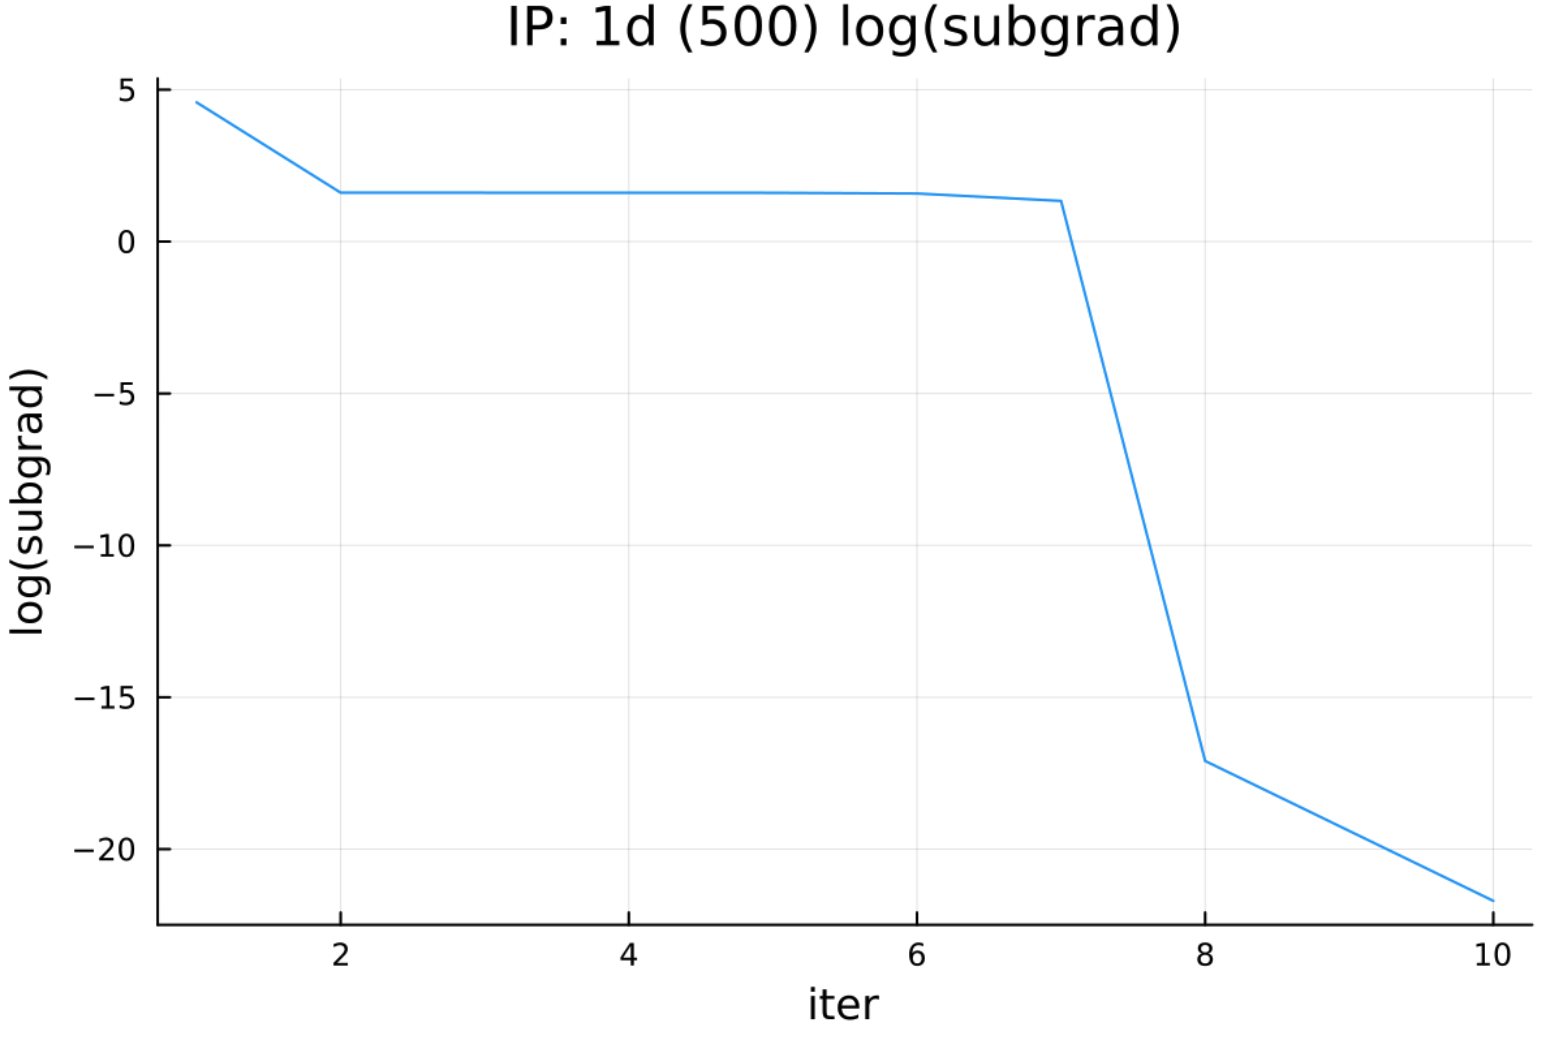
\includegraphics[width=0.3\textwidth]{Interior Point Method/subgradplot3_fig/IP1dloggrad.png}		 	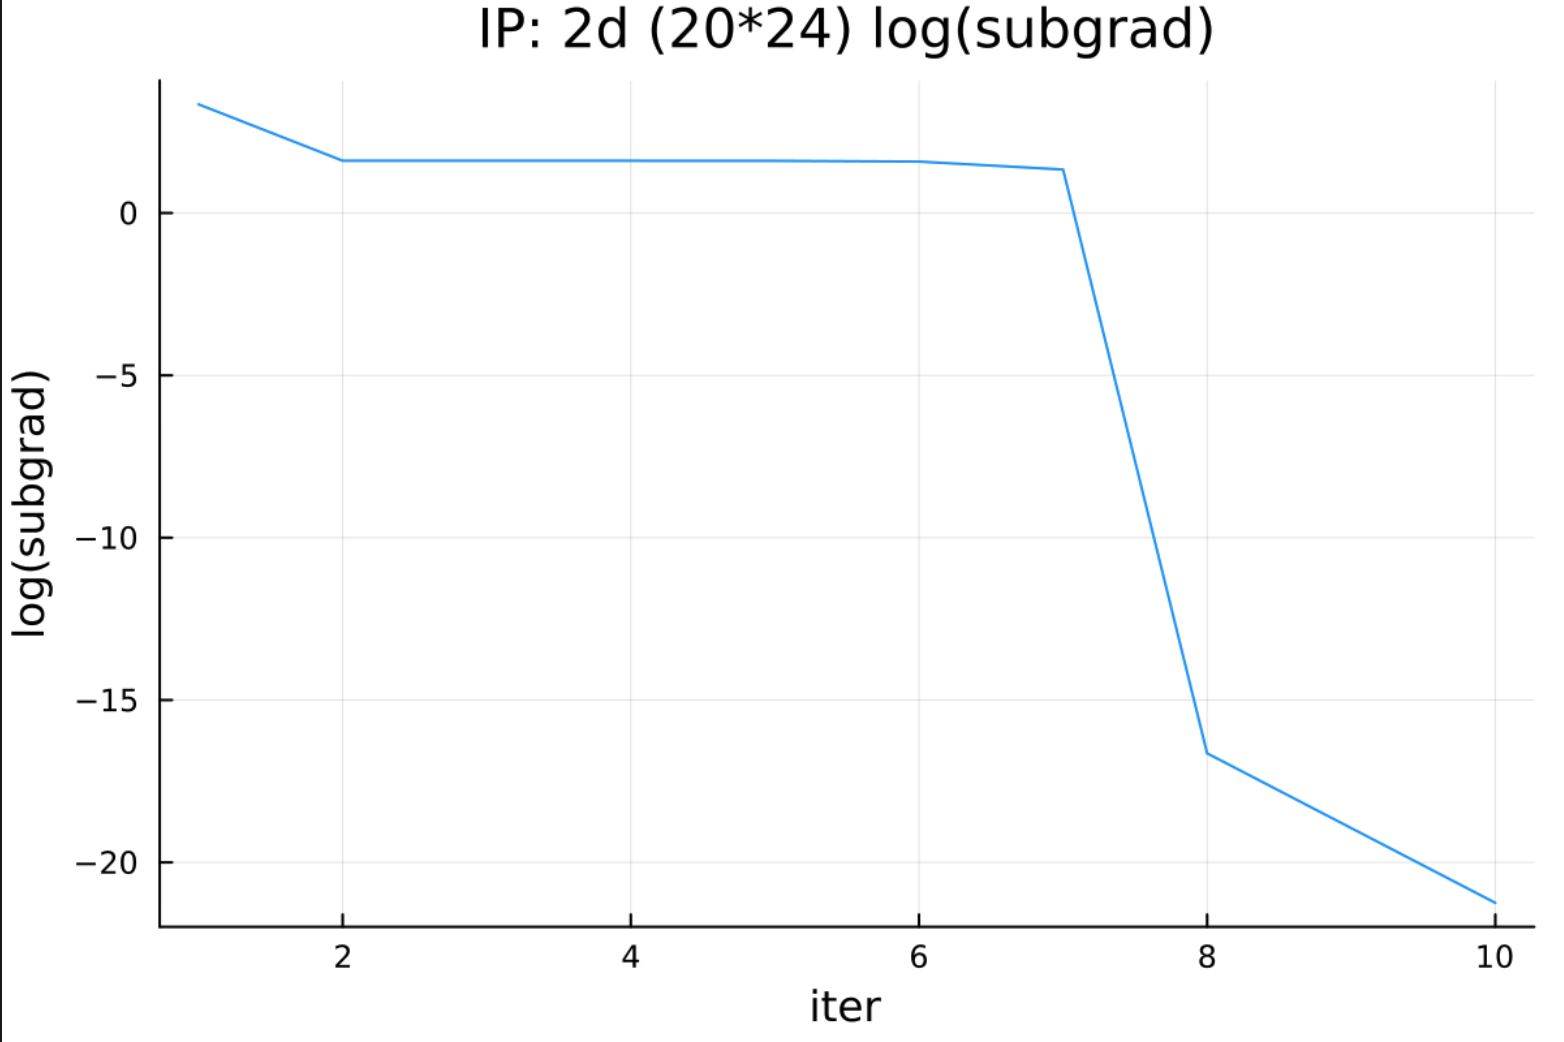
\includegraphics[width=0.3\textwidth]{Interior Point Method/subgradplot3_fig/IP2dloggrad.png}           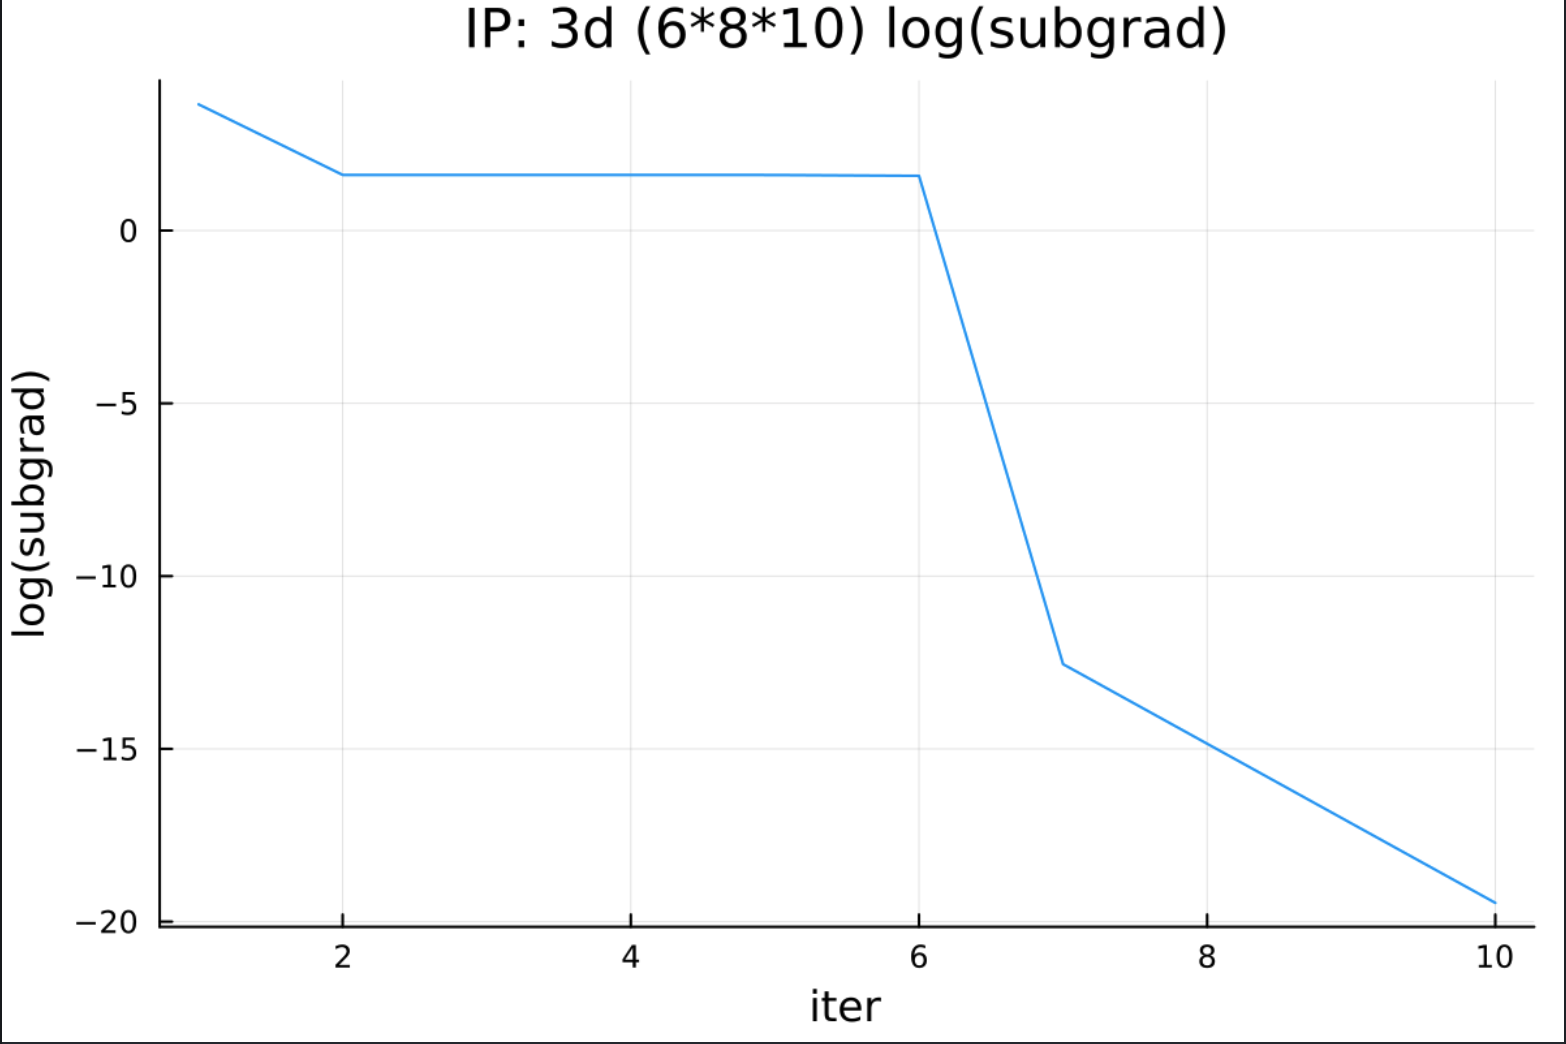
\includegraphics[width=0.3\textwidth]{Interior Point Method/subgradplot3_fig/IP3dloggrad.png}
    		\end{minipage}
      \caption{IP: log(subgrad) vs iter}
		}  
\end{figure}

%References
%\printbibliography
%\appendix



\end{document}
